\let\RaggedRight\raggedright
\let\raggedright\relax
\documentclass[utf8,9pt,mathserif,usepdftitle=false]{beamer}
\usepackage[russian]{babel}

\newcommand{\dd}{\mathrm{d}}
\renewcommand{\Re}{\operatorname{Re}}
\renewcommand{\Im}{\operatorname{Im}}
\renewcommand{\exp}{\operatorname{e}}
\renewcommand{\imath}{\mathrm{i}}

% \input{present.daf}

% \setbeameroption{show notes on second screen}
\setbeameroption{hide notes}
\mode<presentation>
{
  \usetheme{default}
  %\usecolortheme{default} % dove, beaver
  \usecolortheme{whale}
  %\usefonttheme{serif}
}

\hypersetup{%
  pdfinfo={%
    Title={Lyapunov conference, IDSTU},%
    Subject={Spin degrees of freedom for fermion systems},%
    Author={Даниил Кучеров},%
    Keywords={fermion polarization;fermion spinor projection}%
  }
}

\title{Зависимость вероятности выживания электронного нейтрино от углов
  смешивания}%
\author{\underline{Кучеров Д.А.}\\[7em]\raggedleft\footnotesize Научный руководитель:
  Ломов В.П.\\%
}%
\date[ИГУ, 2025]{\vfill%\\[4ex]%
  \small{}Иркутск, 2025}

\begin{document}
\begin{frame}
  \titlepage
\end{frame}

\begin{frame}
	\frametitle{Задачи работы}
  В работе поставлено несколько задач:
  \begin{itemize}
  \item<2-> Изучить теорию нейтринных осцилляций в среде.
  \item<3-> Провести вычисления с помощью метода разложения Магнуса, варьируя значения углов смешивания.
  \item<4-> Проанализировать полученные решения.
  \end{itemize}
\end{frame}

\begin{frame}
	\frametitle{Теоритическая часть}%
	Нейтрино --- нейтральные частицы, имеющие полуцелый спин относящиеся к классу лептонов. Феноменологически выделяют два типа нейтрино: участвующие во взаимодействии --- флейворные и участвующие в распространении в пространстве --- массивные.

  \onslide<1->%
	Нейтрино существуют в трех флейворах: электронные, мюонные и
  тау-нейтрино. Каждый флейвор ассоциируется с соответствующим лептоном
  (электроном, мюоном и тау-лептоном).

  \onslide<2->%
 Самая необычная черта нейтрино — это их осцилляции. Осцилляции нейтрино — периодические переходы между флейворами этих частиц, распространяющихся в веществе или в вакууме. Осцилляции нейтрино возможны благодаря их ненулевым, отличным друг от друга массам.
\end{frame}

\begin{frame}
	\frametitle{Уравнения нейтринных осцилляций}%
    Для случая распространения нейтрино в вакууме массивные состояния нейтрино подчиняются уравнению
    \begin{equation}
        H|\nu_{i}(t)\rangle=\imath\frac{\dd}{\dd t}|\nu_{i}(t)\rangle=
        E_{k}|\nu_{i}(t)\rangle.
    \end{equation}
    Если решение этого уравнения подставить в формулу для смешивания нейтрино получаем соотношение для эволюции флейвора во времени
    \begin{equation}
        |\nu_{\alpha}(t)\rangle=\sum_{i}U_{\alpha i}^{*}\exp^{-\imath E_{k}t}|\nu_{i}\rangle.
    \end{equation}

    В случае распространения нейтрино в среде, ее влияние можно описать в терминах потенциалов, в
  которых распространяются нейтрино, зависящим от состава среды, электрической
  нейтральности, намагниченности (ориентации спинов), скоростей частиц
  среды. Учитывая данные обстоятельства, было выведено уравнение:
	\begin{equation}\label{eq:2}
		\imath\frac{\dd\psi}{\dd\xi}=[H_{0}+\nu(\xi)W]\psi
	\end{equation}
	Оно имеет несколько особенностей: уравнение матричное, состоящее из трёх
  компонент, \(H(\xi)=[H_{0}+\nu(\xi)W]\) это унитарная матрица гамильтониана
  эволюции.  Данное уравнение на сегодняшний день не имеет аналитического
  решения. А численное интегрирование достаточно трудоёмкий процесс.
\end{frame}

\begin{frame}
	\frametitle{Генерирование и обработка данных}%
  Для численного решения уравнения будет использован метод разложения Магнуса, а конкретно, алгоритм M4.
  Для автоматизации процесса генерации и обработки данных были написаны сценарии в bash-оболочке. Уравнение нейтринных осцилляций было численно решено с помощью программы m4-tol.
\end{frame}

\begin{frame}
  \begin{figure}[h]
		\centering
		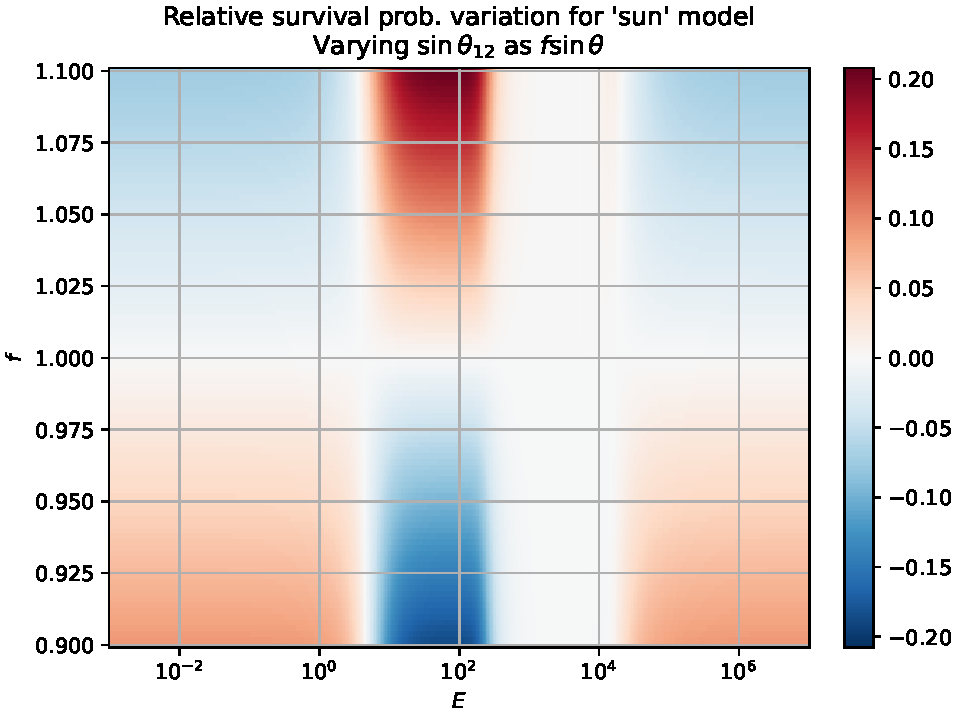
\includegraphics[width=0.8\linewidth]{sun-in-ang12}
		\caption{График относительного отклонения \(\langle P_{ee}\rangle\) при вариации угла \(\Theta_{12}\) }
	\end{figure}
\end{frame}

\begin{frame}
	\begin{figure}[h]
		\centering
		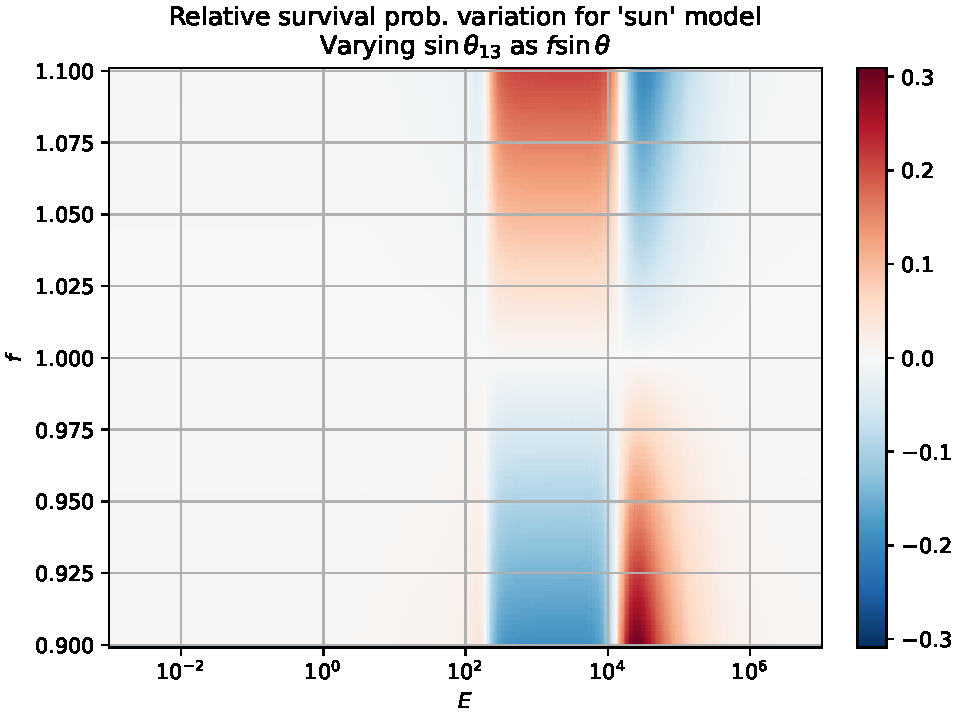
\includegraphics[width=0.8\linewidth]{sun-in-ang13}
		\caption{График относительного отклонения \(\langle P_{ee}\rangle\) при вариации угла \(\Theta_{13}\)}
	\end{figure}
\end{frame}

\begin{frame}

	\frametitle{Вывод}
    \begin{itemize}
        \item<1-> Разобран механизм осцилляций в вакууме и среде.
        \item<2-> Разработаны сценарии для автоматизации расчётов и визуализации данных.
    \end{itemize}
\end{frame}
\begin{frame}
    \frametitle{Перспективы}
    \begin{itemize}
        \item<1-> Провести анализ для других типов нейтрино.
        \item<2-> Провести анализ с вариацией параметров профиля плотности.
        \item<3-> Разработать формулы для анализа корреляций в вариациях.
    \end{itemize}
\end{frame}
\begin{frame}
  \frametitle{КОНЕЦ}
  \LARGE\centering\bfseries
  СПАСИБО ЗА ВНИМАНИЕ!
\end{frame}

\begin{frame}
  \frametitle{Дополнительный материал}
\end{frame}

\end{document}

%%% Local Variables:
%%% mode: latex
%%% fill-column: 80
%%% TeX-master: t
%%% TeX-PDF-mode: t
%%% End:
%%% vim: syn=tex ft=tex tw=80 ts=2 sw=2 et:
